\documentclass[10pt,journal,compsoc]{IEEEtran}

\ifCLASSOPTIONcompsoc

  \usepackage[nocompress]{cite}
\else

  \usepackage{cite}
\fi

\ifCLASSINFOpdf
\usepackage[pdftex]{graphicx}
\usepackage{caption}
\graphicspath{{./images/}}
\DeclareGraphicsExtensions{.jpeg,.png}

\usepackage{hyperref}
\hypersetup{
    colorlinks=true,
    linkcolor=blue,
    filecolor=magenta,      
    urlcolor=cyan,
}
\urlstyle{same}
\else

\fi

\newcommand\MYhyperrefoptions{bookmarks=true,bookmarksnumbered=true,
pdfpagemode={UseOutlines},plainpages=false,pdfpagelabels=true,
colorlinks=true,linkcolor={black},citecolor={black},urlcolor={black},
pdftitle={Embedded Systems Project},%<!CHANGE!
pdfsubject={Journal IEEE Project},%<!CHANGE!
pdfauthor={Duverley Grajales},%<!CHANGE!
pdfkeywords={Stm32 microcontroller, Heart Rate Sensor, Gps, Gsm, Accelerometer, Battery}}%<^!CHANGE!

\hyphenation{op-tical net-works semi-conduc-tor}

\begin{document}

\title{Heart Rate monitoring, Fall detection and Alarming system with data storage in MicroSD}

\author{Grajales~Q.~Duverley~A.,~\IEEEmembership{Student~S227324,~Polito}

\thanks{Manuscript received October 24, 2016; revised ...}}

\markboth{Journal \LaTeX\ IEEE}
{}

\IEEEtitleabstractindextext{%
\begin{abstract}
In the final years the patient health monitoring, has played an important paper for researchers in Embedded Systems. The goal is develop a reliable health monitoring system portable able to measure Heart Rate, proper acceleration (to detect a fallen) and the location from GPS also send SMS to predefined numbers (using Gsm module) and write periodically the condition to microSD.\\
The Embedded System will be designed for patients that need a constant periodically monitoring by family or doctor but does not have a critical condition. If the system detect a critical condition send an SMS with GPS location alerting to predefined numbers for bring a quick service.
\end{abstract}

\begin{IEEEkeywords}
Stm32f4 microcontroller, Heart Rate Sensor, Gps, Accelerometer, Gsm, Lithium Battery.
\end{IEEEkeywords}}

\maketitle

\IEEEdisplaynontitleabstractindextext

\IEEEpeerreviewmaketitle


\ifCLASSOPTIONcompsoc
\IEEEraisesectionheading{\section{Introduction}\label{sec:introduction}}
\else
\section{Introduction}
\label{sec:introduction}
\fi

\IEEEPARstart{H}{ealth} is one of the global challenges for humanity. According to the constitutions of World Health Organization (WHO) the highest attainable standard of health is a fundamental right for an individual. Healthy individuals lead to secure their lifetime income and hence to increase in
gross domestic product and in tax revenues. Healthy individuals also reduce pressure on the
already overwhelmed hospitals, clinics, and medical professionals and reduce workload on the
public safety networks, charities, and governmental (or non-governmental) organizations. To
keep individuals healthy an effective and readily accessible modern healthcare system is a
prerequisite.

\hfil

\section{Caracteristics of the Embedded system}

The portable embedded system will have the following characteristics:

\begin{itemize}
  \item Know the location of the patient periodically 
  \item Check periodically the Heart Rate of the patient
  \item Detect a fallen of the patient
  \item Send SMS to predefined numbers
  \item Create card based patient data monitoring
\end{itemize}

\hfil

With which the embedded system will be able to create an alarming system based in Hear Rate monitoring and fall detection, which will send an SMS with the patient location to predefined numbers (family, doctor, clinic, etc...) if detect a critical condition. This first functionality is illustrated in Fig. 1.

\begin{figure}[h]
  \centering
  \captionsetup{justification=centering}
  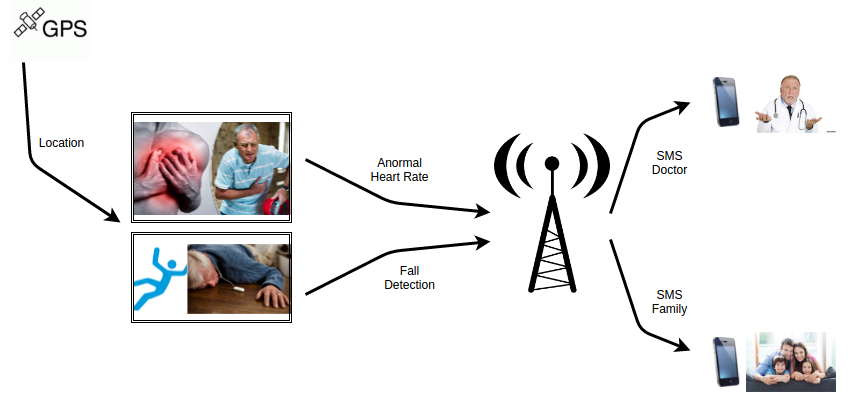
\includegraphics[scale=.30]{es0}
  \caption{Alarming system in a critical condition}
  \label{fig:fig1}
\end{figure}

\hfil

Also create a card based patient data monitoring writing periodially information of the sensors to the microSD. This second functionality is illustrated in Fig. 2.

\begin{figure}[h]
  \centering
  \captionsetup{justification=centering}
  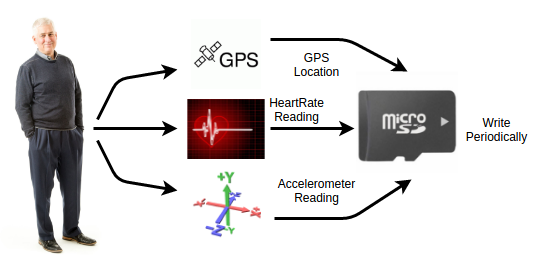
\includegraphics[scale=.40]{es1}
  \caption{Card based patient data monitoring}
  \label{fig:fig2}
\end{figure}

\hfil

\section{Embedded system to develop}

To implement the functions listed above, will be need use a microcontoller able to do:

\begin{itemize}
  \item Read location from GPS
  \item Read ADCs for X, Y and Z from Triple Axis Accelerometer
  \item Read ADC from HeartRate Sensor
  \item Send SMS using GSM modem
  \item Write periodically to microSD
\end{itemize}

\hfil

The embedded system is illustrated in Fig. 3.

\begin{figure}[h]
  \centering
  \captionsetup{justification=centering}
  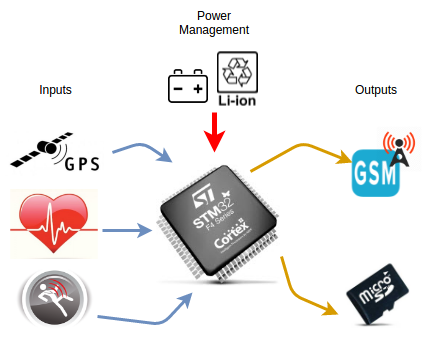
\includegraphics[scale=.50]{es2}
  \caption{Embedded System Inside}
  \label{fig:fig3}
\end{figure}

\hfil

In the next subsections, will be explained each part of the embedded system:

\hfil

\subsection{Microcontroller}
Will be used a microcontroller with the balance between performance, power efficiency and integrated peripherals to avoid problems in the future. After searching the good microcontrollers available today the best option is \href{http://www.st.com/en/microcontrollers/stm32f446re.html}{stm32f446re} of the STMicroelectronics. The main features of the microcontroller is illustrated in Fig. 4.

\begin{figure}[h]
  \centering
  \captionsetup{justification=centering}
  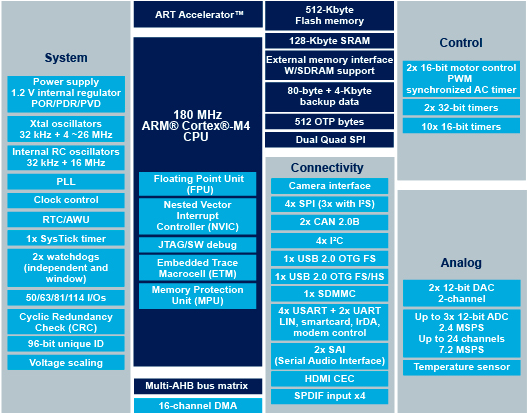
\includegraphics[scale=.45]{es3}
  \caption{Characteristics of the STM32F446}
  \label{fig:fig4}
\end{figure}

\hfil

The important is that can begin to build a prototype with the \href{http://www.st.com/en/evaluation-tools/nucleo-f446re.html}{Nucleo stm32f446re} board, which have the programmer incorporated. The Nucleo STM446 Board is illustrated in Fig. 5.

\begin{figure}[h]
  \centering
  \captionsetup{justification=centering}
  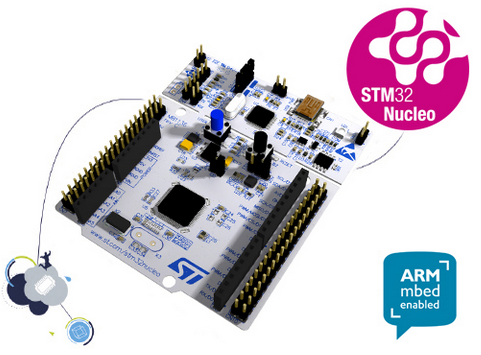
\includegraphics[scale=.45]{es4}
  \caption{Nucleo STM446 Board}
  \label{fig:fig5}
\end{figure}

\hfil

In summary:

\begin{itemize}
  \item 1x UART GSM Module
  \item 1x UART GPS Sensor
  \item 1x SPI Accelerometer Sensor
  \item 1x SPI microSD Card
  \item 1x ADC Heart Rate Sensor
\end{itemize}

\hfil

\subsection{GPS Sensor}

There are two good options in the market, which are:

\begin{enumerate}[\IEEEsetlabelwidth{2)}]

\item LS2003H-G of the \href{http://www.locosystech.com}{LOCOSYS} company, is a complete standalone GNSS smart antenna module. The LS2003H-G Module is illustrated in Fig. 6.

\begin{figure}[h]
  \centering
  \captionsetup{justification=centering}
  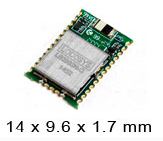
\includegraphics[scale=.45]{es5}
  \caption{LS2003H-G Module}
  \label{fig:fig6}
\end{figure}

\hfil

In which the main features of LS2003H-G are:

\begin{itemize}
  \item Support 99-channel GPS
  \item Capable of SBAS (WAAS, EGNOS, MSAS, GAGAN)
  \item Support GPS, GLONASS, GALILEO and QZSS
  \item Low power consumption
  \item Indoor and outdoor multi-path detection and compensation
  \item SMD type with stamp holes; RoHS compliant
  \item Up to 10 Hz update rate
\end{itemize}

\hfil

\item NEO-M8N of the \href{https://www.u-blox.com/en}{u-blox} company, is a concurrent GNSS module. The NEO-M8N Module is illustrated in Fig. 7.

\begin{figure}[h]
  \centering
  \captionsetup{justification=centering}
  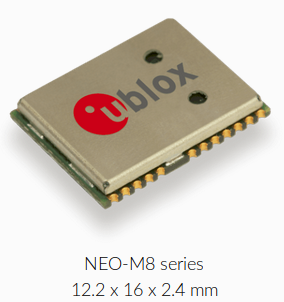
\includegraphics[scale=.45]{es6}
  \caption{NEO-M8N Module}
  \label{fig:fig7}
\end{figure}

\hfil

In which the main features of NEO-M8N are:

\begin{itemize}
  \item Concurrent reception of up to 3 GNSS (GPS, Galileo, GLONASS, BeiDou)
  \item Industry leading –167 dBm navigation sensitivity
  \item Security and integrity protection
  \item Supports all satellite augmentation systems
  \item Advanced jamming and spoofing detection
  \item Product variants to meet performance and cost requirements
  \item Backward compatible with NEO‑7 and NEO‑6 families
\end{itemize}

\end{enumerate}

\hfil

Anyway the communication between the GPS Sensor with microcontroller is UART (Universal Asynchronous Receiver Transmitter).

\hfil

\subsection{Triple Axis Accelerometer Sensor}
There are good options in the market but the \href{http://www.analog.com/en/index.html}{Analog Devices} Company have a \href{http://www.analog.com/en/products/mems/accelerometers.html#accelerometers}{list} of excellent accelerometers, but a good option for this application is ADXL362. The ADXL362 Module is illustrated in Fig. 8.

\begin{figure}[h]
  \centering
  \captionsetup{justification=centering}
  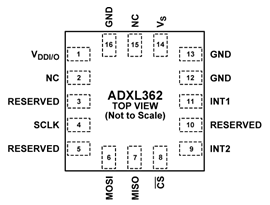
\includegraphics[scale=.45]{es7}
  \caption{ADXL362 Module}
  \label{fig:fig8}
\end{figure}

\hfil

In which the main features of ADXL362 are:

\begin{itemize}
  \item Ultralow power
  \item High resolution: 1 mg/LSB
  \item Built-in features for system-level power savings
  \item Low noise down to 175 μg/√Hz
  \item Wide supply and I/O voltage ranges: 1.6 V to 3.5 V
  \item Acceleration sample synchronization via external trigger
  \item On-chip temperature sensor
\end{itemize}

\hfil

The communication between the Triple Axis Accelerometer Sensor with microcontroller is SPI.

\hfil

\subsection{GMS Module}

There are two good options in the market, which are:

\begin{enumerate}[\IEEEsetlabelwidth{2)}]

\item SIM900 of the \href{http://www.simcom.eu}{SIMCOM} company, is a complete Quad-band GSM/GPRS module in a SMT type and designed with a very powerful single-chip processor. The SIM900 Module is illustrated in Fig. 9.

\begin{figure}[h]
  \centering
  \captionsetup{justification=centering}
  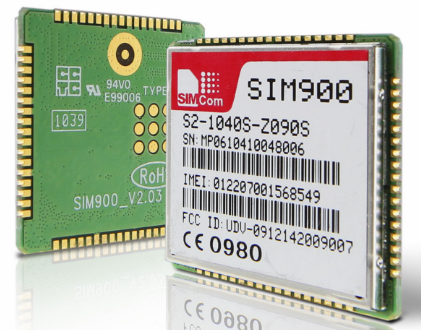
\includegraphics[scale=.45]{es8}
  \caption{SIM900 Module}
  \label{fig:fig9}
\end{figure}

\hfil

In which the main features of SIM900 are:

\begin{itemize}
  \item SIM900 is designed with a very powerful single-chip processor integrating AMR926EJ-S core 
  \item Quad-band GSM/GPRS module with a size of 24mmx24mmx3mm 
  \item SMT type suit for customer application
  \item An embedded Powerful TCP/IP protocol stack 
  \item Based upon mature and field-proven platform, backed up by our support service, from definition to design and production 
\end{itemize}

\hfil

\item M95 of the \href{http://www.quectel.com/default.aspx}{Quectel} company, is one of the smallest Quad-band GSM/GPRS modules, ultra low power consumption and extended temperature range. The M95 Module is illustrated in Fig. 10.

\begin{figure}[h]
  \centering
  \captionsetup{justification=centering}
  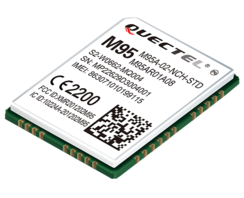
\includegraphics[scale=.45]{es9}
  \caption{M95 Module}
  \label{fig:fig10}
\end{figure}

\hfil

In which the main features of M95 are:

\begin{itemize}
  \item One of the smallest Quad-band GSM/ GPRS modules
  \item Easier soldering process with LCC package
  \item Embedded Class-AB amplifier
  \item Power consumption as low as 1.3mA
  \item QuecFOTA TM
  \item Jamming detection
  \item DTMF decoding
\end{itemize}

\end{enumerate}

\hfil

Anyway the communication between the GSM Module with microcontroller is UART (Universal Asynchronous Receiver Transmitter).

\hfil

\subsection{microSD Card}

Any microSD can be used in this application. For example, microSD card is illustrated in Fig. 11.

\begin{figure}[h]
  \centering
  \captionsetup{justification=centering}
  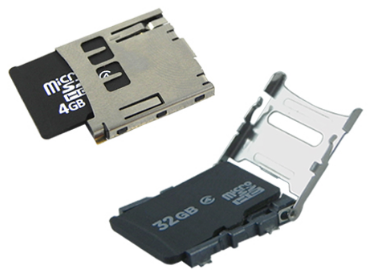
\includegraphics[scale=.45]{es10}
  \caption{microSD Card}
  \label{fig:fig11}
\end{figure}

%

The communication between the microSD Card with microcontroller is SPI.

%

\subsection{Lithium Ion Battery}

Low power embedded system is a challenge for this application, as well as hardware and software optimising for energy efficiency. Will use an energy measurement system that enables to understand the effect of the different improvements. 

First will develop the embedded system to be sure the battery to choose, obviously as the system is portable the type of the battery will be a Lithium Ion Battery. For example, Lithium Ion Battery is illustrated in Fig. 12.

\begin{figure}[h]
  \centering
  \captionsetup{justification=centering}
  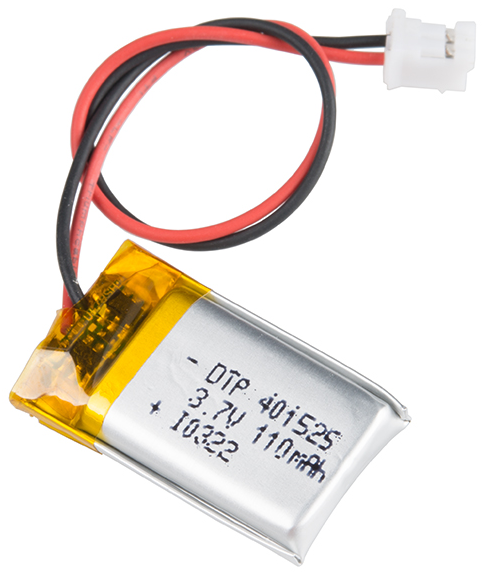
\includegraphics[scale=.3]{es11}
  \caption{Lithium Ion Battery}
  \label{fig:fig12}
\end{figure}

%

Therefore will need a charger that accurately balances and charges Lithium Polymer. A battery charger that could be used is illustrated in Fig. 13.

\begin{figure}[h]
  \centering
  \captionsetup{justification=centering}
  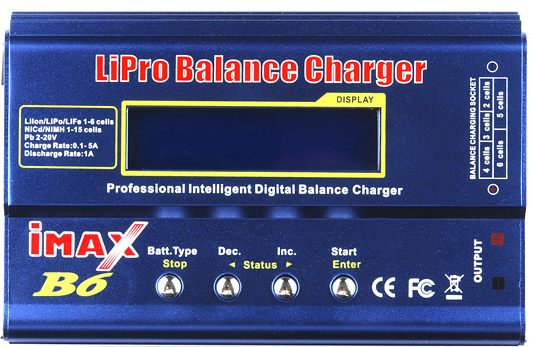
\includegraphics[scale=.35]{es12}
  \caption{Battery Charger}
  \label{fig:fig13}
\end{figure}

%

\subsection{HeartRate Sensor}

Is the difficult decision of this project, choose an appropriate Heart Rate Sensor, three are the alternatives:

\begin{enumerate}[\IEEEsetlabelwidth{3)}]

\item AD8232 of the \href{http://www.analog.com/en/index.html}{Analog Devices} company, is a Single-Lead Heart Rate Monitor Analog Front End. The AD8232 Module is illustrated in Fig. 14.

\begin{figure}[h]
  \centering
  \captionsetup{justification=centering}
  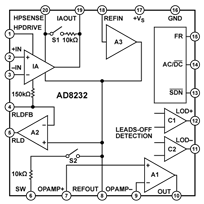
\includegraphics[scale=.45]{es13}
  \caption{AD8232 Module}
  \label{fig:fig14}
\end{figure}

%

But consequently need an electrode pads and biomedical sensor pads in funtion to measure the Heart Rate. The Typical Sensor Placements are illustrated in Fig. 15.

\begin{figure}[h]
  \centering
  \captionsetup{justification=centering}
  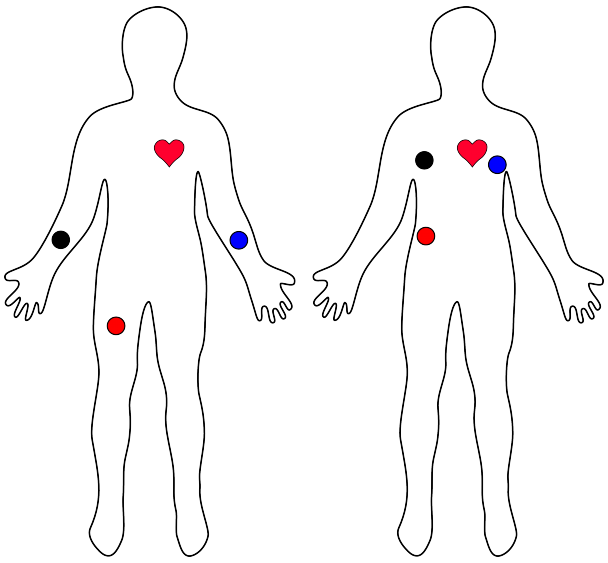
\includegraphics[scale=.35]{es14}
  \caption{Typical Sensor Placements}
  \label{fig:fig15}
\end{figure}

%

\item APDS-9008 of the \href{http://www.avagotech.com}{Avago Technologies} company, is a Miniature Surface-Mount Ambient Light Photo Sensor in order to use, need a linear operational amplifier as MCP6001  of Microchip. The APDS-9008 Module is illustrated in Fig. 16.

\begin{figure}[h]
  \centering
  \captionsetup{justification=centering}
  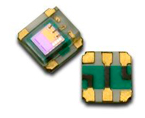
\includegraphics[scale=.45]{es15}
  \caption{APDS-9008 Module}
  \label{fig:fig16}
\end{figure}

%

But consequently to measure the Hear Rate is different to the previous sensor. The Sensor Placements are illustrated in Fig. 17.

\begin{figure}[h]
  \centering
  \captionsetup{justification=centering}
  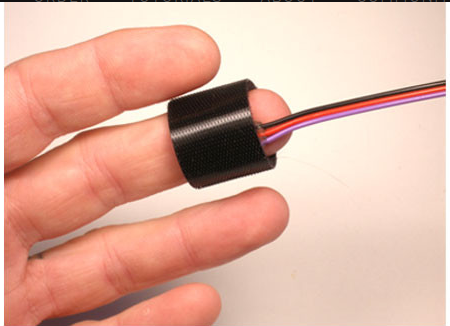
\includegraphics[scale=.45]{es16}
  \caption{ypical Sensor Placements}
  \label{fig:fig17}
\end{figure}

%

\item RMCM01 Polar OEM receiver of the \href{https://www.polar.com/it}{Polar} company, is a heart rate monitor chip which is able to decode the signal coming from the popular Polar heart rate belts.  It is able to decode both coded and uncoded belts. The RMCM01 Polar OEM receiver is illustrated in Fig. 18.

\begin{figure}[h]
  \centering
  \captionsetup{justification=centering}
  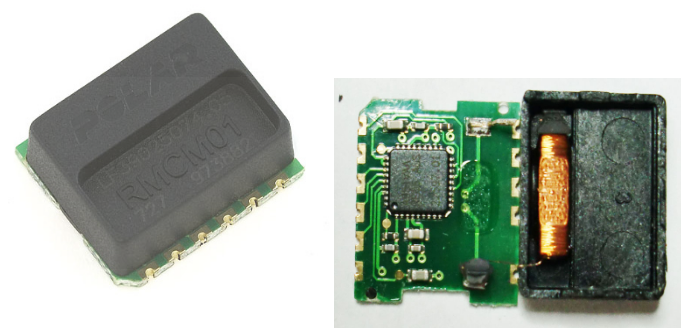
\includegraphics[scale=.30]{es17}
  \caption{RMCM01 Polar OEM receiver}
  \label{fig:fig18}
\end{figure}

%

But consequently to measure the Hear Rate is different to the previous sensor. The Sensor Placements are illustrated in Fig. 19.

\begin{figure}[h]
  \centering
  \captionsetup{justification=centering}
  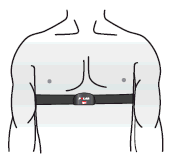
\includegraphics[scale=.45]{es18}
  \caption{Polar Sensor Placements}
  \label{fig:fig19}
\end{figure}

%

Anyway an Analog to Digital Converter (ADC) will be necessary in order to communicate with the microcontroller.

\end{enumerate}

%\hfill \break

\section{Conclusion}

\begin{itemize}
  \item The ideal system will has a significantly reduced size and weight, which improves its versatility and mobility.
  \item Any abnormalities in health conditions are informed via SMS to the indicated mobile number through GSM in order to create an alarming system.
  \item The healthcare family and professional can know news about their patients from a remote location at any time with their location.
  \item Create a reliable card based patient data monitoring.
  \item A low cost portable and power efficient Embedded System.
\end{itemize}
  
\end{document}
